\newcommand<>\highlightbox[2]{%
  \alt#3{\makebox[\dimexpr\width-2\fboxsep]{\colorbox{#1}{#2}}}{#2}%
}
\definecolor{chal-poison}{HTML}{1e78b4}\newcommand{\chpoison}[2][1-]{\highlightbox<#1>{chal-poison!50}{#2}}
\definecolor{chal-qual}{HTML}{ff7f0f}\newcommand{\chqual}[2][1-]{\highlightbox<#1>{chal-qual!50}{#2}}
\definecolor{chal-decent}{HTML}{2da02d}\newcommand{\chdecent}[2][1-]{\highlightbox<#1>{chal-decent!50}{#2}}
\definecolor{chal-feat}{HTML}{d62727}\newcommand{\chfeat}[2][1-]{\highlightbox<#1>{chal-feat!50}{#2}}
\definecolor{chal-hetero}{HTML}{9567bd}\newcommand{\chhetero}[2][1-]{\highlightbox<#1>{chal-hetero!50}{#2}}
\definecolor{chal-unknown}{HTML}{8d574b}\newcommand{\chunknown}[2][1-]{\highlightbox<#1>{chal-unknown!50}{#2}}
\definecolor{chal-transfer}{HTML}{e377c3}\newcommand{\chtransfer}[2][1-]{\highlightbox<#1>{chal-transfer!50}{#2}}
\definecolor{chal-comm}{HTML}{7f7f7f}\newcommand{\chcomm}[2][1-]{\highlightbox<#1>{chal-comm!50}{#2}}



% \subsection[\slr Systematic Literature Review]{\texorpdfstring{\circled{contrib/slr}{S}~Federated Intrusion Detection Systems}{Federated Intrusion Detection Systems}}

% \begin{frame}[plain]
%   \subsectionpage
  
%   \footcite*{lavaur_tnsm_2022}
%   \footcite*{lavaur_cesar_2022}
%   \footcite*{lavaur_icdcs_demo_2024}
% \end{frame}

\begin{frame}{Case Study}
  \bigskip
  \textbf{Collaborating with Federated Intrusion Detection Systems (FIDSs)}:
  \begin{itemize}[<+->]
    \item Each organization has its own NIDS\footnotemark{} and monitors an information system.
    \item Objective: improve their local detection performance.
    \item Means: \alert{expert knowledge} (\ie, datasets) and \alert{computing resources} (\ie, model training).
  \end{itemize}
  % \only<1>{\footnotetext[1]{Network Intrusion Detection System}}
  \onslide<+->
  \begin{columns}
    \column{.5\textwidth}
    \textbf{A cross-silo use case}~\autocite{kairouz_AdvancesOpenProblems_2021}:
    \begin{itemize}
      \item few clients (\ie, 10--100);
      \item substantial amount of data, high heterogeneity;
      \item high availability, significant computing resources.
    \end{itemize}

    \onslide<+->
    \column{.5\textwidth}
    \vspace{-1.5em}
    \begin{figure}
      \centering
      \resizebox{.8\linewidth}{!}{\input{figures/thesis/intro/year_histogram.pgf}}
      \caption{Publications on FL \& IDS (until 2024-04). 1600+ results on Scopus in 2026-02.}
    \end{figure}
  \end{columns}

  \alt{\footcite*{kairouz_AdvancesOpenProblems_2021}}{\blankfootnote{\newline}}
  % \begin{figure}
  %   \centering
  %   \makebox[\textwidth][c]{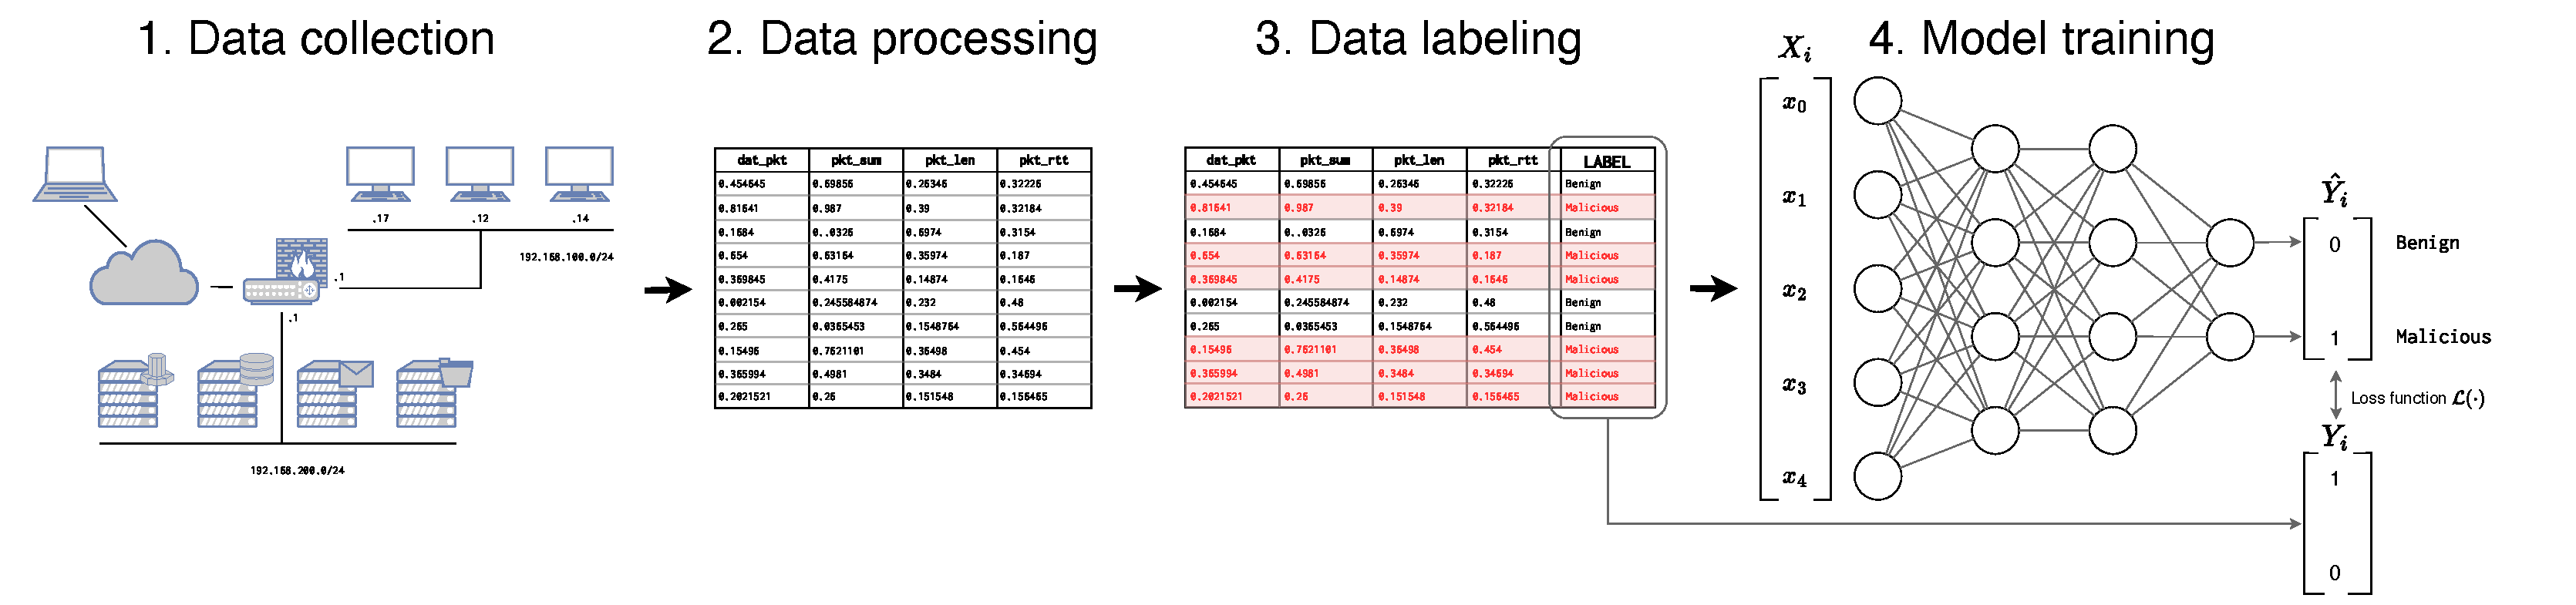
\includegraphics[width=.9\textwidth]{figures/thesis/intro/mlp-workflow.pdf}}
  %   \caption{Typical workflow for ML-based NIDSs.}
  % \end{figure}
\end{frame}

% \begin{frame}{Systematic Literature Review}
  
%   \begin{columns}
%     \begin{column}{.45\textwidth}
%       % \textbf{Systematic Literature Review (SLR)}~\autocite{lavaur_tnsm_2022}
%       % \begin{itemize}
%       %   \item Booming topic over the last 4--5 years.
%       %   \item Very heterogeneous venues and communities.
%       % \end{itemize}

%       \textbf{Challenges from the Literature}~\autocite{lavaur_tnsm_2022}
%       \begin{itemize}[<+->]
%         \item \textit{Functionality}: \chqual[6-]{performance}, \chhetero[6-]{heterogeneity}, \chtransfer[6-]{transferability}, self-defense, and self-healing.
%         \item \textit{Deployment}: \chunknown[6-]{adaptability} and \chdecent[6-]{scalability}.
%         \item \textit{Security and reliability}: \chpoison[6-]{security}, privacy, \chpoison[6-]{trust}, and reputation.
%         \item \textit{Experimentation}: evaluation.
%       \end{itemize}
%     \end{column}
%     \begin{column}{.55\textwidth}
%       \only<5-6>{%
%         \begin{figure}
%           \centering
%           \resizebox{\linewidth}{!}{\input{figures/thesis/intro/challenges_histogram.pgf}}
%           \caption{Challenges addressed by the literature (until 2024-04).}
%         \end{figure}
%       }
%       \only<7>{%
%         \begin{figure}
%           \centering
%           \resizebox{\linewidth}{!}{\input{figures/thesis/intro/year_histogram.pgf}}
%           \caption{Publications on FL \& IDS (until 2024-04). 1600+ results on Scopus in 2026-02.}
%         \end{figure}
%       }
%     \end{column}
%   \end{columns}

%   \footcite*{lavaur_tnsm_2022}
% \end{frame}


\newcommand<>\mktransparent[2]{\alt#3{\texttransparent{#1}{#2}}{#2}}

\begin{frame}{Addressed Challenges}
  
  \begin{columns}
    \begin{column}{.5\textwidth}
      \begin{figure}
        \centering
        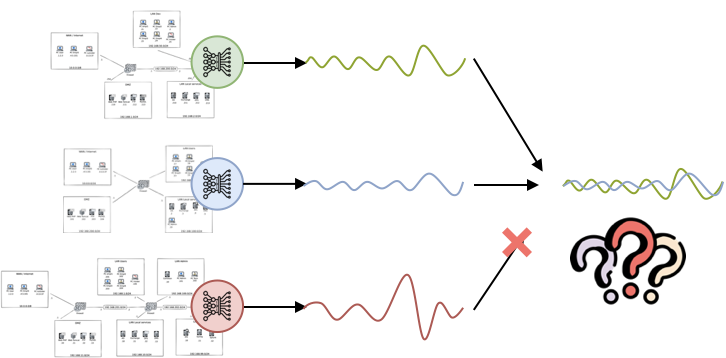
\includegraphics[width=\linewidth]{figures/thesis/intro/heterogeneity.png}
        \caption{Heterogeneity headaches.}
      \end{figure}
    \end{column}

    \begin{column}{.5\textwidth}
      \mktransparent<2->{0.5}{%
      \textbf{Challenge I}: \textit{Too much heterogeneity leads to poor performance\dots}~\autocite{lavaur_icdcs_demo_2024}
      }

      \medskip
      \mktransparent<1,3>{0.5}{%
      \textbf{Challenge II}: \textit{Difficult to identify malicious contributions when models are different\dots}
      }
      
      \medskip
      \mktransparent<1-2>{0.5}{%
      \textbf{Challenge III}: \textit{No representative dataset of heterogeneous distributed intrusion detection\dots}~\autocite{lavaur_cesar_2022}
      }
    \end{column}
  \end{columns}

  \only<1>{\footcite*{lavaur_icdcs_demo_2024}}
  \only<2>{\blankfootnote{\newline}}
  \only<3>{\footcite*{lavaur_cesar_2022}}
  
\end{frame}